\documentclass[mathserif,serif]{beamer}
\usepackage[utf8]{inputenc}
\usepackage{tikz}
\usetikzlibrary{calc}

\title{Weierstrass' Approximation Theorem and Bernstein Polynomials}
\author{Jishnu Kaiwar
  \and
  Bing En Gan
  \and
  Constantinos Azas}
\date{May 2019}
\subject{Mathematics}


\begin{document}
\frame{\titlepage}

\begin{frame}
  \frametitle{Approximating functions with polynomials.}
  \begin{itemize}
  \item<+-> Is it possible?
  \item<+-> Where is it possible?
  \item<+-> What do we mean by approximate?

  \end{itemize}
\end{frame}

\begin{frame}
  \frametitle{History of the Problem}
  \begin{itemize}
  \item 1885: Karl Weierstrass (1815-1897) establishes his Approximation Theorem, provides a general proof.
  \item 1908: Charles Poussin poses the question: \emph{Can we approximate functions with $n$-degree polynomials with an error less than $\frac{1}{n}$?}
  \item 1911: Sergei Bernstein solves this problem using \emph{Probability Theory}.
  \end{itemize}
\end{frame}

\begin{frame}{Bernstein Polynomials}
We know by the definition of Taylor's theorem that it is used to approximate functions around fixed points in an interval. According to Weierstrass approximation theorem, it looks unsuitable to use Taylor's theorem. In this case we use Bernstein polynomials and their properties.    
\end{frame}

\begin{frame}{Weierstrass approximation theorem}
\begin{theorem}[Weierstrass approximation theorem]
If $F(x)$ is any continuous function in the interval $[0,1]$, it is always possible, regardless how small $\epsilon$, to determine a polynomial $E_n=a_0x^n+a_1x^{n-1}+\dots+a_n$ of degree $n$ high enough such that we have
\begin{equation*}
    |F(x)-E_n(x)|<\epsilon
\end{equation*}
for every point in the interval under consideration.
\end{theorem}
\end{frame}

\begin{frame}{Definition}
A Bernstein basis polynomial, degree $n$ is defined by
\begin{equation}
\label{eq:bp:1}
 B_{i,n}(x)=\binom{n}{i}x^i(1-x)^{n-i} 
\end{equation}
The Bernstein polynomial of a function $f$ is defined by:
\begin{equation}
B_n(f)=B_n(t;f)=\sum_{i=0}^nf(\frac{i}{n})B_{i,n}(t)   
\end{equation}    
\end{frame}
\begin{frame}{Bernstein Polynomials under a graph}
\begin{figure}
\centering
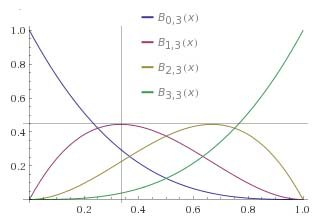
\includegraphics[width=95mm]{BP.jpg}
\caption{Graph of Bernstein Polynomial of degree 3}
\label{fig:1}
\end{figure}    
\end{frame}
\begin{frame}{Higher Degree Bernstein Polynomials}
\begin{figure}
\centering
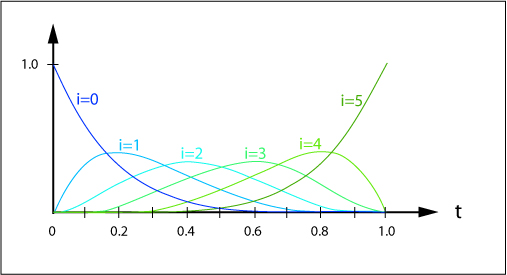
\includegraphics[width=95mm]{BP5.jpg}
\caption{Graph of Bernstein Polynomial of degree 5}
\end{figure} 
\end{frame}
\begin{frame}{Properties of Bernstein polynomials}
\begin{theorem}[Recursive definition]
We can consider a basis of degree n and can be defined as the sum of two Bernstein polynomials of degree $n-1$.
\begin{equation*}
B_{i,n}(t)=(1-t)B_{i,n-1}(t)+tB_{i-1,n-1}(t)    
\end{equation*}
\end{theorem}
\end{frame}
\begin{frame}{Properties of Bernstein polynomials}
\begin{theorem}[Positivity]
Bernstein basis polynomials are all considered positive if we take them in the interval $[0,1]$ and strictly positive on the interval $(0,1)$.
\end{theorem}    
\end{frame}
\begin{frame}{Properties of Bernstein polynomials}
\begin{theorem}[Bernstein polynomials form a partition of unity]
Consider a set of funtions $f_i(t)$. this is said to be a partition of unity if and only if their sum is equal to $1$ for all values of $t$. So, the $k + 1$ Bernstein basis polynomials for a Bernstein polynomial of degree $k$ form a partition of unity. That is:
\begin{equation*}
B_k(t)=\sum_{i=0}^nB_{i,n}(t)= B_{0,n}(t)+B_{1,n}(t)+...+B_{n,n}(t)=1,
\end{equation*}
for $0\leq t\leq 1$  
\end{theorem}    
\end{frame}

\begin{frame}
  \frametitle{B\'ezier Curves}
  \begin{itemize}
  \item<+-> $\mathbf{r}(t) := \sum_{i=0}^{n} B_{i,n}(t) \mathbf{b}_i$
  \item<+-> $r, b_i \in \mathbb{R}^2$ and $B_{i,n}(t)$ is the Bernstein basis.
  \item<+-> The B\'ezier Curve lies in the convex hull of its basis points.
\end{itemize}
 \end{frame}

\begin{frame}
  \frametitle{A Linear B\'ezier Curve}
  \begin{figure}
  \centering
  \begin{tikzpicture}
    \filldraw
    (0,0) circle (1pt) node [left] {$\mathbf{b}_0$} --
    (1.5,1) circle (1pt) node [below] {$\mathbf{r}(\frac{1}{2})$} --
    (3,2) circle (1pt) node [right] {$\mathbf{b}_1$};
  \end{tikzpicture}
  \caption{$\mathbf{r}(t) = \mathbf{b}_0 (1 - t) + \mathbf{b}_1 t$}
\end{figure}
\end{frame}

\begin{frame}
  \frametitle{A Cubic B\'ezier Curve}
\begin{figure}
  \centering
  \begin{tikzpicture}
    \coordinate (A) at (0,0);
    \coordinate (B) at (2,3);
    \coordinate (C) at (5,3);
    \coordinate (D) at (4,0);
    \draw (A) .. controls (B) and (C) .. (D);
    \filldraw [dotted]
    (A) circle (1pt) node [left] {$\mathbf{b}_0$} --
    (B) circle (1pt) node [left] {$\mathbf{b}_1$};
    \filldraw [dotted]
    (C) circle (1pt) node [right] {$\mathbf{b}_2$} --
    (D) circle (1pt) node [right] {$\mathbf{b}_3$};
  \end{tikzpicture}
  \caption{$\mathbf{r}(t) = (1-t)^3 \mathbf{b}_0 + t(1-t)^2 \mathbf{b}_1 + t^2(1-t) \mathbf{b}_2 + t^3 \mathbf{b}_3$}
\end{figure}
\end{frame}

\begin{frame}
  \frametitle{B\'ezier Curves}
  \begin{figure}
  \centering
  \begin{tikzpicture}
    \coordinate (A) at (0,0);
    \coordinate (B) at (3,6);
    \coordinate (C) at (6,7);
    \coordinate (D) at (10,2);
    \coordinate (h01) at ($0.5*(A) + 0.5*(B)$);
    \coordinate (h12) at ($0.5*(B) + 0.5*(C)$);
    \coordinate (h23) at ($0.5*(C) + 0.5*(D)$);
    \coordinate (h012) at ($0.5*(h01) + 0.5*(h12)$);
    \coordinate (h123) at ($0.5*(h12) + 0.5*(h23)$);
    \coordinate (c) at ($0.5*(h012) + 0.5*(h123)$);
    \draw (A) .. controls (B) and (C) .. (D);
    \draw [gray]
    (A) circle (1pt) node [left] {$\mathbf{b}_0$} --
    (h01) circle (1pt) node [left] {$\mathbf{h}_{01}$} --
    (B) circle (1pt) node [left] {$\mathbf{b}_1$} --
    (h12) circle (1pt) node [above] {$\mathbf{h}_{12}$} --
    (C) circle (1pt) node [right] {$\mathbf{b}_2$} --
    (h23) circle (1pt) node [right] {$\mathbf{h}_{23}$} --
    (D) circle (1pt) node [right] {$\mathbf{b}_3$};
    \filldraw[dotted]
    (h01) circle (1pt) --
    (h012) circle (1pt) node [left] {$\mathbf{h}_{012}$} --
    (h12) circle (1pt);
    \filldraw[dotted]
    (h12) circle (1pt) --
    (h123) circle (1pt) node [right] {$\mathbf{h}_{123}$} --
    (h23) circle (1pt);
    \filldraw[dotted]
    (h012) circle (1pt) --
    (c) circle (1pt) node [above] {$\mathbf{c}$} --
    (h123) circle (1pt);
  \end{tikzpicture}
\end{figure}
\end{frame}

\begin{frame}{Weierstrass approximation theorem}
\begin{theorem}[Weierstrass approximation theorem]
If $F(x)$ is any continuous function in the interval $[0,1]$, it is always possible, regardless how small $\epsilon$, to determine a polynomial $E_n=a_0x^n+a_1x^{n-1}+\dots+a_n$ of degree $n$ high enough such that we have
\begin{equation*}
    |F(x)-E_n(x)|<\epsilon
\end{equation*}
for every point in the interval under consideration.
\end{theorem}
\end{frame}

\begin{frame}{Bernstein's Probabilistic Proof}
Consider an event $A$, where
$$\mathbb{P}(A)=x$$
Consider a continuous function $F$.
\newline 
Assume $n$ experiments are conducted and the player is paid the sum $F(\frac{m}{n})$ if the event $A$ occurs $m$ times.    
\end{frame}

\begin{frame}{Probabilistic Proof}
Now, calculate the expected value of the money received by the player.
\begin{equation*}
      E_n =:E(F(\frac{m}{n})) = \sum_{m=0}^{n} F \left( \frac{m}{n} \right) \binom{m}{n} x^n (1-x)^{n-m}
\end{equation*}
Note that this is a polynomial with degree $n$.
\end{frame}

\begin{frame}{Probabilistic Proof}
End goal:
\begin{equation*}
    |F(x)-E_n(x)|<\epsilon
\end{equation*}
\end{frame}

\begin{frame}{Probabilistic Proof}
By definition of continuity, we have:
\begin{equation*}
    (\exists\delta>0)(|x-x_0|<\delta)\implies(\forall\epsilon>0)(|F(x)-F(x_0)|<\frac{\epsilon}{2})
\end{equation*}
\end{frame}

\begin{frame}{Step 1}
Consider $|x-\frac{m}{n}|<\delta$.
\newline
Let $\overline{F}(x)$ be the maximum and $\underline{F}(x)$ be the minimum of $F(x)$ for $x$ in this interval.
\newline
Now consider $|x-\frac{m}{n}|>\delta$.
\newline
Set the maximum of $|F(x)|$ in this interval be $L$.
\newline
Then, let $\eta$ be the probability such that $|x-\frac{m}{n}|>\delta$. Conversely, the probability that the inequality is $|x-\frac{m}{n}|<\delta$ is $(1-\eta)$.
\end{frame}

\begin{frame}{Step 2}
Looking back at the function $E_n$,
\begin{align*}
    E_n(x) &= \mathbb{E}\left(F\left(\frac{m}{n}\right)\cdot1\right) \\
    &= \mathbb{E}\left(F\left(\frac{m}{n}\right)\cdot(\eta+(1-\eta))\right) \\
    &= \mathbb{E}\left(F\left(\frac{m}{n}\right)\cdot \mathbb{I}\left[|x-\frac{m}{n}|>\delta\right]\right) + \mathbb{E}\left(F\left(\frac{m}{n}\right)\cdot \mathbb{I}\left[|x-\frac{m}{n}|<\delta\right]\right)\\
\end{align*}
\end{frame}

\begin{frame}{Step 3}
So, we have the following inequality,
\begin{align*}
    -L\cdot\eta&<\mathbb{E}\left(F\left(\frac{m}{n}\right)\cdot \mathbb{I}\left[|x-\frac{m}{n}|>\delta\right]\right)<L\cdot\eta\\
    \underline{F}(x)\cdot(1-\eta)&<\mathbb{E}\left(F\left(\frac{m}{n}\right)\cdot \mathbb{I}\left[|x-\frac{m}{n}|<\delta\right]\right)<\overline{F}(x)\cdot (1-\eta)
\end{align*}
Combining both inequalities, 
\begin{equation}\label{ineq1}
 \underline{F}(x)\cdot(1-\eta)-L\cdot\eta<E_n(x)<\overline{F}(x)\cdot (1-\eta)+L\cdot\eta 
\end{equation}
\end{frame}

\begin{frame}{Step 4}
By the law of large numbers from probability theory, we have that
\begin{equation*}
    \frac{m}{n}\longrightarrow x \;\;\text{as}\;\;n \rightarrow \infty
\end{equation*}
Hence, $\eta$ tends to zero.
\newline
Therefore, we can take $n$ large enough such that 
\begin{equation*}
\eta<\frac{\epsilon}{4L}
\end{equation*}
\end{frame}

\begin{frame}{Step 5}
Going back to the inequality(\ref{ineq1}) and rearranging,
\begin{equation*}
 \underline{F}(x)\cdot(1-\eta)-L\cdot\eta<E_n(x)<\overline{F}(x)\cdot (1-\eta)+L\cdot\eta 
\end{equation*}
\begin{align*}
    F(x)+(\underline{F}(x)-F(x))-\eta(L+\underline{F}(x))<E_n(x)< &F(x)+(\overline{F}(x)-F(x))\\
    &+\eta(L-\overline{F}(x))
\end{align*}
And so,
\begin{equation*}
    F(x)-\frac{\epsilon}{2}-\frac{2L}{4L}\epsilon<E_n(x)<F(x)+\frac{\epsilon}{2}+\frac{2L}{4L}\epsilon
\end{equation*}
\end{frame}

\begin{frame}{Conclusion}
Hence, we get
\begin{equation*}
    |F(x)-E_n(x)|<\epsilon
\end{equation*}
Since we know $E_n$ is clearly a polynomial with degree $n$, so the theorem is proved.
\end{frame}


\end{document}

%%% Local Variables:
%%% mode: latex
%%% TeX-master: t
%%% End:
